\begin{appendix}
%You can use an appendix for optional proofs or details of your evaluation which are not absolutely necessary to the core understanding of your paper. 
\section{proofs}
\subsection{Proof of Theorem Monotonic}

\begin{proof}
	\label{sec:app:proof:monotonic}
	It is known that $\Delta Y^k=F(\Delta X^k)$and $\Delta X^0=X^0$.
	\begin{align}
	&G\Big(\Delta Y^0\cup (F\circ G)(\Delta Y^0)\cup\ldots\cup (F\circ G)^k(\Delta Y^0)\Big)\notag \\
	=&G\Big(G(\Delta Y^0)\cup (F\circ G)(\Delta Y^0)\cup \ldots \cup (F\circ G)^k( \Delta Y^0)\Big)\tag{2}\\
	=&G\Big(F\circ G(\Delta Y^0)\cup (F\circ G)^2(\Delta Y^0)\cup \ldots \cup (F\circ G)^k(\Delta Y^0)\Big) \tag{3}\\
	=& \ldots \notag \\
	=&G\Big((F\circ G)^k(\Delta Y^0)\Big)\tag{4}\\
	=&(G \circ F)^{k+1}(X^0).\notag
	\end{align}
	Line 3 is true because of the accumulative property. Due to the monotonic property line 4 is true .By repeat applying these two properties, we can reduce the original formula to line 5, the result of normal recursive aggregation. 
\end{proof}

\subsection{Proof of Theorem Asynchronous}
 \begin{proof}
 \label{sec:app:proof:correct}
 In this proof, We assumed that $X$ can be divided into two disjoint subset $X_0$ and $X_1$. we exchange the subset belongs to any two  recursion, and then prove that they have the same formula with the origin form. This is the basic form which can generalize all the other situations.
 \begin{align}
 &G(\Delta X^0\cup \ldots \cup F\circ G(\Delta X^{i}_0 \cup \Delta X^{j}_1)\cup\ F\circ G(\Delta X^{j}_0 \cup \notag\\ &\Delta X^{i}_1) \ldots\cup \Delta X^n)\tag{1} \\
 =&G( \ldots \cup G \circ F\circ G(\Delta X^{i}_0 \cup \Delta X^{{j}}_1)\cup\ G \circ F\circ G(\Delta X^{{j}}_0 \cup \notag\\ &\Delta X^{i}_1) \ldots)\tag{2} \\
 =&G( \ldots \cup G \circ F(\Delta X^{i}_0 \cup \Delta X^{{j}}_1)\cup\ G \circ F(\Delta X^{{j}}_0 \cup \Delta X^{{i}}_1) \ldots)\tag{3} \\
  =&G( \ldots \cup (G\circ F(\Delta X^{i}_0) \cup G\circ F(\Delta X^{{j}}_1))\cup\ (G \circ F(\Delta X^{{j}}_0) \notag\\ &\cup G \circ F(\Delta X^{i}_1)) \ldots )\tag{4} \\
  =&G( \ldots \cup (G\circ F(\Delta X^{i}_0) \cup G\circ F(\Delta X^{i}_1))\cup\ (G \circ F(\Delta X^{{j}}_0) \notag\\ &\cup G  \circ F(\Delta X^{{j}}_1)) \ldots )\tag{5} \\
  =&G( \ldots \cup G \circ F(\Delta X^{i}_0 \cup \Delta X^{{i}}_1)\cup\ G \circ F(\Delta X^{{j}}_0 \cup \Delta X^{{j}}_1) \ldots)\tag{6} \\
  =&G( \ldots \cup F \circ G(\Delta X^{i}_0 \cup \Delta X^{{i}}_1)\cup\ F \circ G(\Delta X^{{j}}_0 \cup \Delta X^{{j}}_1) \ldots)\tag{7} \\
=&G(\ldots \cup F \circ G(\Delta X^i)\cup\ F \circ G(\Delta X^{j}) \ldots\cup \Delta X^n).\tag{8}
 \end{align}

By applying the \textbf{accumulative} property and \textbf{order indenpendent} property, we can have line 2, 3. Line 4 is true because of \textbf{accumulative} property
and \textbf{distributive} property, line (5,6) is because of the \textbf{community} property. line (7)can be obtained by applying \textbf{order independent} property again.
Line 8 is the formula of synchronous accumulative recursive aggregation. Since the difference between $i$ and $j$ can be arbitrary large, the computation need to iterative infinity.
 \end{proof}
 \subsection{Proof of Theorem Convertibility}
 \label{sec:app:proof:convert}
 \begin{proof}
 Since we have $\Delta X^0=X^1-X^0$.
 \begin{align}
&G^+(X^0\cup \Delta X^0 \cup G^+\circ F'(\Delta X^0)\cup \ldots (G^+ \circ F')^{k-1}(\Delta X^0 )) \notag\\
=&G^+(X^1 \cup G^+\circ F'(\Delta X^0  )\cup \ldots (G^+ \circ F')^{k-1}(\Delta X^0  )) \notag\\
=&G^+(G^+(X^1\cup G^+\circ F'(\Delta X^0  ))\cup \ldots (G^+ \circ F')^{k-1}(\Delta X^0 )) \tag{3}\\
=&G^+(G\circ F(X^1)\cup \ldots (G^+ \circ F')^{k-1}(\Delta X^0 )) \tag{4}\\
=&\ldots \notag\\
=&G^+((G\circ F)^{k-2}(X^1)\cup(G^+ \circ F')^{k-1}(\Delta X^0 )) \notag\\
=&G\circ F(X^{k-1})\tag{6}
 \end{align}
Line 3 is true because of the \textbf{accumulative} property.Line 4 is true because the second condition of Theorem \ref{th:convert}. After repeat applying these two property, we can obtain line 6 which is the synchronous recursive program formula. 
 \end{proof}
 

 \section{Datalog Examples}
 \label{sec:app:example}
 
 \begin{verbatim}
 Program 3. Connected Components
 \end{verbatim}\vspace{-0.1in}\small
 \begin{lstlisting}
 r1. cc(X,X)$\leftarrow$ edge(X,_).
 r2. cc(Y,min[$v$])$\leftarrow$ cc(X,$v$),edge(X,Y),
                    cc(Y,$v$).
 \end{lstlisting}
 \normalsize
 
 Program 3 computes the connected components in a graph. Each vertex starts as its own connected component with its identifier. For all combinations of facts that satisfy the recursive bodies, the aggregate function \texttt{min} keeps and propagates only the current minimal component ID $v$ for each vertex \texttt{Y}.
  \begin{comment}
\begin{verbatim}
Program 4. Single Source Shortest Path
\end{verbatim}
\vspace{-0.1in}
\small
\begin{lstlisting}
r1. sssp(X,$d$)$\leftarrow$ X=1,$d=0$.
r2. sssp(Y,min[$d$])$\leftarrow$ sssp(X,$d1$),edge(X,Y,$d2$),
$d=d1+d2$,sssp(Y,$d$).
\end{lstlisting}
\normalsize

In Program 4, rule \texttt{r1} initializes the predicate \texttt{sssp} by specifying the source node $X=1$ and the shortest distance from source as $d=0$. \texttt{r2} is a recursive rule since it has the \texttt{sssp} predicate in both its head and body. \texttt{r2} will recursively produce \texttt{sssp} fact by joining the old \texttt{sssp} and \texttt{edge}. If there is a path from source to $X$ of length $d_1$ and an edge from $X$ to $Y$ of length $d_2$, there is a path from source to $Y$ with length $d=d_1+d_2$. If there is already a path to $Y$ found before, it should be also considered. Hence, the shortest distance from source to $Y$ is updated by the minimum of these possible distances, i.e., min$[d]$. The recursion will terminate as soon as no shortest distance is updated.
 
 
 \begin{verbatim}
 Program 5. Max Probability Path
 \end{verbatim}\vspace{-0.1in}\small
 \begin{lstlisting}
 r1. reach(X,Y,$P$) $\leftarrow$ net(X,Y,$P$).
 r2. reach(X,Y,max[$P$]) $\leftarrow$ reach(X,Z,$P1$),
                          reach(Z,Y,$P2$),
                          $P=P1*P2$,
                          reach(X,Y,$P$).
 \end{lstlisting}
 \normalsize
 
 Program 5 \cite{7113340} computes the max probability path between two nodes in a network. The \texttt{net} predicate denotes the probability \texttt{P} of reaching \texttt{Y} from \texttt{X}.
 
 \begin{verbatim}
 Program 6. Least Common Ancestor
 \end{verbatim}\small
 \begin{lstlisting}
 r1. ancestor(Y,X,1) $\leftarrow$ cite(Y,X), X<seed.
 r2. ancestor(Z,X,min[$d$]) $\leftarrow$ ancestor(Z,Y,$d'$),
                             cite(Y,X),$d=d'+1$,
                             ancestor(Z,X,$d$).
 r3. LCA(p1,p2,min[max(  $\leftarrow$ ancestor(p1,X,d1),
 d1,d2)],year,X)          ancestor(p2,X,d2),
                          Paper(X,year),
                          p1<p2.
 \end{lstlisting}
 \normalsize
 
 Program 6 \cite{Wang:2015:AFR:2824032.2824052} computes the least common ancestor (LCA) for pairs of publications in a citations graph. An ancestor a of a paper \texttt{Z} is any paper that is transitively cited by \texttt{Z}, and the LCA a of two papers \texttt{X} and \texttt{Y} is the least ancestor of both \texttt{X} and \texttt{Y}.
 
 \begin{verbatim}
 Program 7. What is the cost of each part
 \end{verbatim}\vspace{-0.1in}\small
 \begin{lstlisting}
 r1. cost(Part,$\mathcal{C}$) $\leftarrow$ basic(Part,cost).
 r2. cost(Part,sum[$\mathcal{C}$]) $\leftarrow$ assb(Part,Sub,$n$),
                                    cost(Sub,$c$),
                                    $\mathcal{C}=c*n$,
                                    cost(Part,$\mathcal{C}$).
 \end{lstlisting}
 \normalsize
 
 Program 7 \cite{7113340} is for computing the cost of a part from the cost of its subparts. The \texttt{assb} predicate denotes each part¡¯s required subparts and number required, and basic denotes the part¡¯s cost.
 
 \begin{verbatim}
 Program 8. Viterbi Algorithm
 \end{verbatim}\vspace{-0.1in}\small
 \begin{lstlisting}
 r1. calcV(0,X,max($L$)) $\leftarrow$ s(0,EX),p(X,EX,$L1$),
                          pi(X,$L2$),$L=L1*L2$.
 r2. calcV($T$,Y,max[$L$]) $\leftarrow$ s($T$,EY),p(Y,EY,$L1$),
                            $T1=T-1$,t(X,Y,$L2$),
                            calcV($T1$,X,$L3$),
                            $L=L1*L2*L3$.
 \end{lstlisting}
 \normalsize
 
 Program 8 \cite{7113340} is the Viterbi algorithm for hidden Markov models. \texttt{t} denotes the transition probability \texttt{L2} from state \texttt{X} to \texttt{Y}; \texttt{s} denotes the observed sequence of length \texttt{L+1}; \texttt{p} denotes the likelihood \texttt{L1} that state \texttt{X (Y)} emitted \texttt{EX (EY)}. \texttt{r1} finds the most likely initial observation for each \texttt{X}. \texttt{r2} finds the most likely transition for observation \texttt{T} for each \texttt{Y}.
 
 \begin{verbatim}
 Program 9. Who will come to the party?
 \end{verbatim}\small
 \begin{lstlisting}
 r1. coming(X) $\leftarrow$ sure(X).
 r2. coming(X) $\leftarrow$ cntComing(X,$N$), $N\geq 3$.
 r3. cntComing(Y,count[*]) $\leftarrow$ friend(Y,X),
                            coming(X).
 \end{lstlisting}
 \normalsize
 
 In this program, some people will come to the party for sure, whereas others only join when at least three of their friends are coming. Program 9 \cite{7113340} describes the retrieving process. With \texttt{cntComing}, each person watches the number of their friends that are coming grow, and once that number reaches three, the person will then come to the party too.
 
 \begin{verbatim}
 Program 10. Galaxy Evolution
 \end{verbatim}\small
 \begin{lstlisting}
 r1. galaxies(1,gid) $\leftarrow$ galaxies_seed(gid).
 r2. galaxies(t+1,gid2) $\leftarrow$ galaxies(t,gid1),
                         edges(t,gid1,gid2,c),
                         c$\geq$threshold.
 r3. edges(t,gid1,gid2, $\leftarrow$ galaxies(t,gid1),
 count[*])               particles(pid,gid1,t),
                         particles(pid,gid2,t+1).
 \end{lstlisting}
 \normalsize
 
 Program 10 \cite{Wang:2015:AFR:2824032.2824052} computes the history of a set of galaxies in an astrophysical simulation. The history of a galaxy is the set of past galaxies that merged over time to form the galaxy of interest at present day. The predicate \texttt{Particles(pid,gid,t)} holds the simulation output as a set of particles, where \texttt{pid} is a unique particle identifier, and \texttt{gid} is the identifier of the galaxy that the particle belongs to at time \texttt{t}. The \texttt{gid} values are unique only within their timesteps \texttt{t}, but a particle retains the same \texttt{pid} throughout the simulation.
 
 
 \begin{verbatim}
 Program 11. Belief Propagation
 \end{verbatim}\small
 \begin{lstlisting}
 r1. G(v,0) $\leftarrow$ E(v,_,_).
 r2. B(v,c,b) $\leftarrow$ E(v,c,b).
 r3. G(t,i) $\leftarrow$ G(s,i-1),A(s,t,w),$\neg$G(t,_).
 r4. B(t,c2,sum[b']) $\leftarrow$ G(t,i),A(s,t,w),
                     B(s,c1,b),
                     G(s,i-1),H(c1,c2,h),
                     b'=w*b*h,
                     [sum$[\Delta b']<T$];
 \end{lstlisting}
 \normalsize
 
 Belief Propagation \cite{910572} is a message-passing algorithm for performing inference on graphical models, such as Bayesian networks and Markov random fields. In Program 11, \texttt{B} is the to-be-returned beliefs, \texttt{G} maintains the geodesic numbers, \texttt{A} is an input weighted network with initial beliefs \texttt{E}, and \texttt{H} is the coupling scores. \texttt{r3} and \texttt{r4} should be repeated evaluated where the geodesic number \texttt{i} is increasing, and stops when no more facts inserted into \texttt{G}. Note that, the shown Datalog program describes a single-pass belief propagation process since it does not allow loopy propagation (by $\neg$\texttt{G(t,\_)} in \texttt{r3}) \cite{Gatterbauer:2015:LSB:2735479.2735490}.
 
 \begin{verbatim}
 Program 12. SimRank
 \end{verbatim}\small
 \begin{lstlisting}
 r1. D(X,count[*]) $\leftarrow$ E(X,Y).
 r2. S(X,Y,1) $\leftarrow$ E(X,Y).
 r3. S(X,Y,sum[s']) $\leftarrow$ S(X',Y',s),E(X,X'),E(Y,Y'),
                    D(X,d1),D(Y,d2),X$\neq$Y,
                    s'=$\frac{C}{d1*d2}$*s,
                    [sum$[\Delta s']<T$].
 \end{lstlisting}
 \normalsize
 
 SimRank algorithm \cite{Jeh:2002:SMS:775047.775126} is an algorithm to evaluate the similarities between node pairs in a graph. In Program 12, \texttt{S} maintains the similarities between node pairs, \texttt{E} is the edge data, \texttt{D} maintains the out degree information. The algorithm terminates when the sum of differences between two recursions is small enough.
 
 \begin{verbatim}
 Program 13. Jacobi Method
 \end{verbatim}\small
 \begin{lstlisting}
 r1. X(i,x) $\leftarrow$ X(i,1).
 r2. C(i,c) $\leftarrow$ A(i,i,$a_{ii}$),B(i,$b_i$),
            c=$\frac{b_i}{a_{ii}}$.
 r3. X(i,sum[x']+c) $\leftarrow$ X(j,x),A(i,j,$a_{ij}$),
                    C(i,c),A(i,i,$a_{ii}$),i$\neq$j,
                    x'=$-\frac{a_{ij}}{a_{ii}}$*x,
                    [sum$[\Delta x']<T$].
 \end{lstlisting}
 \normalsize
 
 In numerical linear algebra, the Jacobi method is a famous iterative algorithm for solving linear equations of the form $A\cdot X=b$, where $A$ is a matrix with each entry $a_{ij}$, and b is a vector with each entry $b_i$. In Program 13, \texttt{X} is the solution vector, \texttt{A} is the matrix, \texttt{B} is the vector, \texttt{C} is a vector maintaining the entry-specific constant $\frac{b_i}{a_{ii}}$. A sufficient (but not necessary) condition for the method to converge is that the matrix \texttt{A} is strictly or irreducibly diagonally dominant, i.e., $|a_{ii}>\sum_{j\neq i}{|a_{ij}|}|$, which implies the convertable condition, so Jacobi Method can be converted and executed asynchronously.
 \end{comment}

\begin{comment}
 \section{More Experiments}
 \label{sec:app:expr}

 \subsection{Effectiveness of Aggregate Operations}
 \label{sec:expr:aggregations}

 \begin{figure}[!t]
 \vspace{-0.1in}
 \centerline{
 \subfloat[RoadCA]{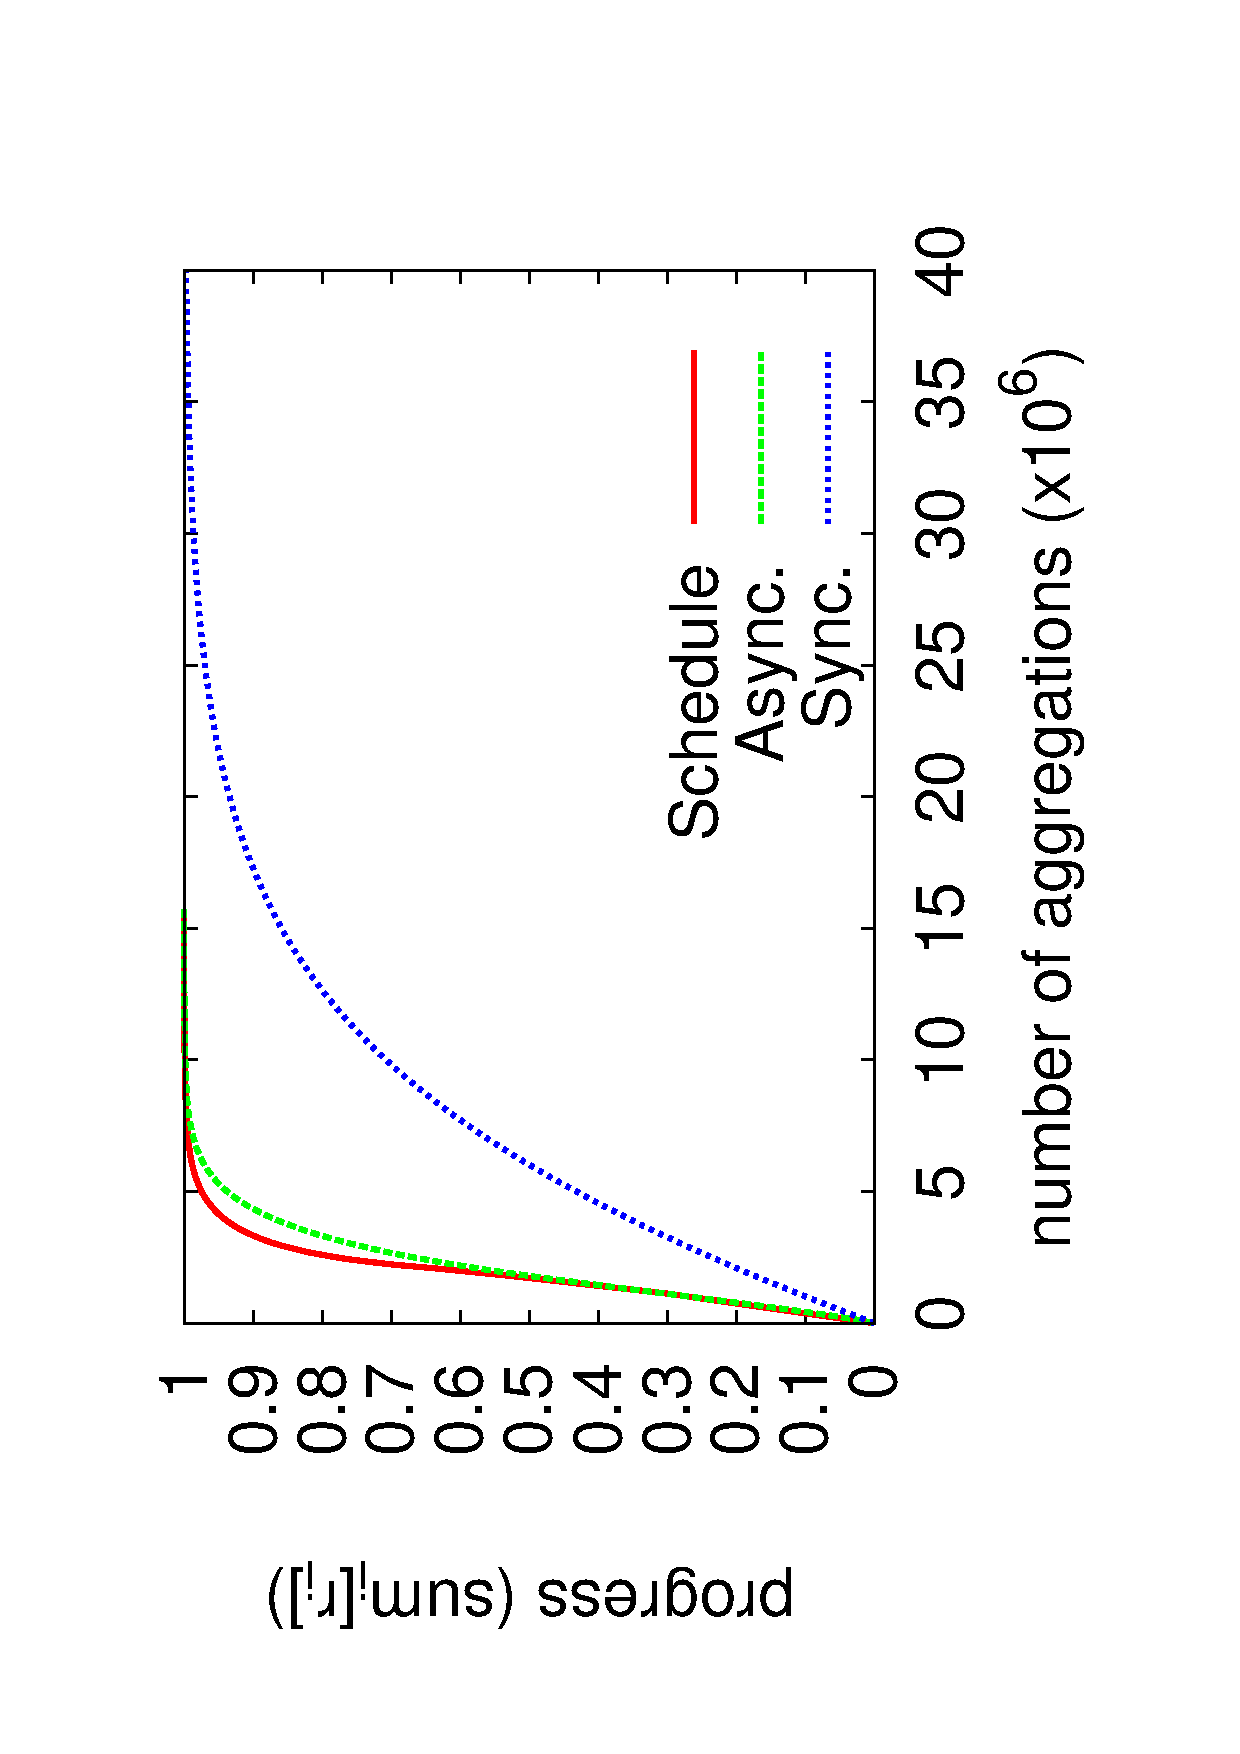
\includegraphics[width=1.3in, angle=-90]{fig/roadca_aggregate_progress}
 \label{fig:single-numagg:roadca}
 \vspace{-0.05in}}
 \hspace{-5mm}
 \subfloat[Livejournal]{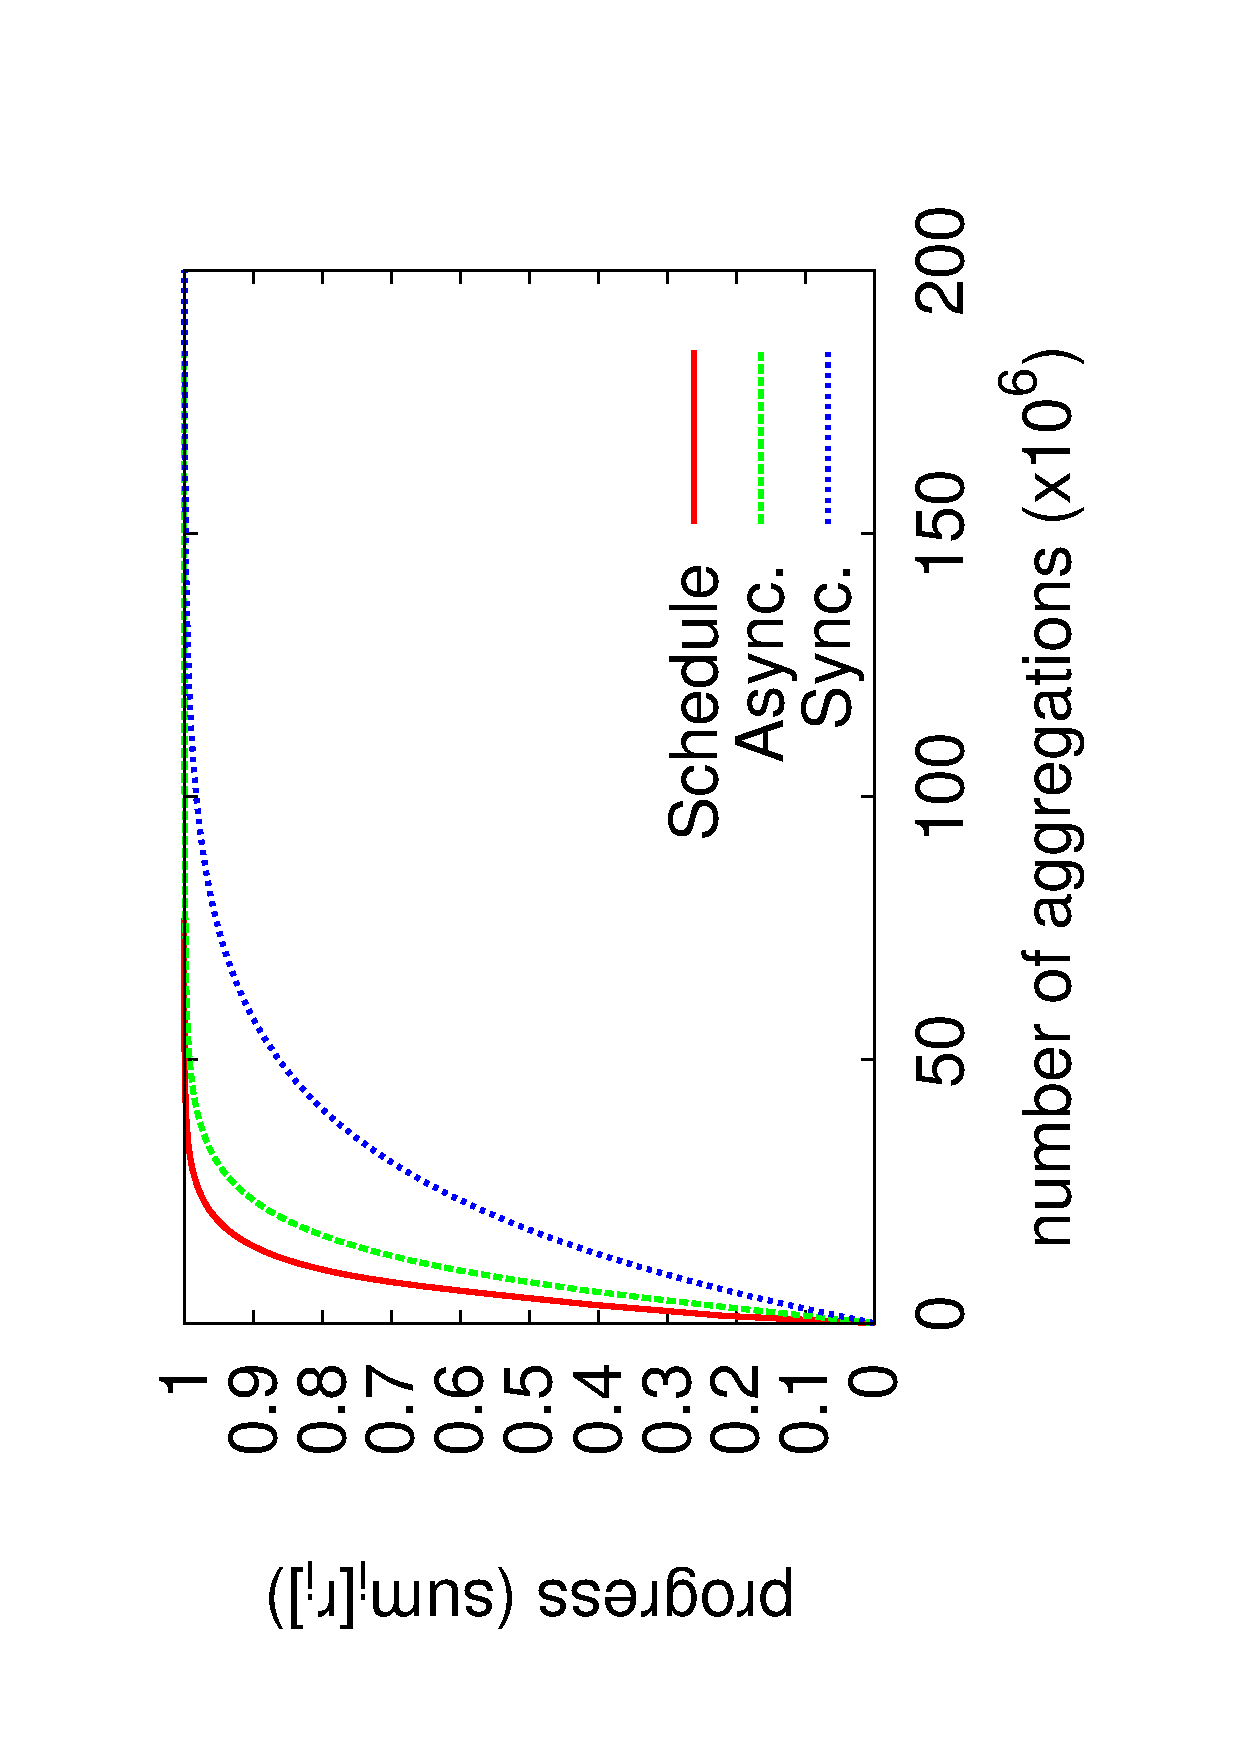
\includegraphics[width=1.3in, angle=-90]{fig/livejournal_aggregate_progress}
 \label{fig:single-numagg:livejournal}
 \vspace{-0.05in}}
 }
 \vspace{-0.1in}
 \caption{Effectiveness of aggregate operations to converging progress}
 \label{fig:single-numagg}
 \vspace{-0.1in}
 \end{figure}
In this experiment, we evaluate the effectiveness of asynchronous aggregations on accelerating the computation prog-ress.
 
 We run PageRank on two datasets, RoadCA and Livejournal, which result in the most speedup and the least speedup comparing to synchronous aggregation as shown in Table \ref{tab:wrokload}. We record the accumulated number of aggregate operations during the computation. In the accumulated version of PageRank (see Sec. \ref{sec:async:convert}), the summation of ranking scores $\sum_i{r_i}$ is approaching to 1 and will finally converge to 1. So we estimate the computation progress by evaluating $\sum_i{r_i}$ periodically. Fig. \ref{fig:single-numagg} shows the results. By using asynchronous aggregation, the converging progress is much faster than using synchronous execution. The scheduling of aggregate operations will further speedup the progress. The asynchronous aggregation with scheduling shows more effectiveness, so that each aggregate operation contributes more. It also shows more effectiveness on the RoadCA graph than on the Lievejournal graph. This is the reason why higher speedup is observed on the RoadCA graph.
\end{comment}
\end{appendix}